% Options for packages loaded elsewhere
\PassOptionsToPackage{unicode}{hyperref}
\PassOptionsToPackage{hyphens}{url}
\documentclass[
  11pt,
  a4paper,
]{article}
\usepackage{xcolor}
\usepackage[margin=22mm,headheight=15pt]{geometry}
\usepackage{amsmath,amssymb}
\setcounter{secnumdepth}{-\maxdimen} % remove section numbering
\usepackage{iftex}
\ifPDFTeX
  \usepackage[T1]{fontenc}
  \usepackage[utf8]{inputenc}
  \usepackage{textcomp} % provide euro and other symbols
\else % if luatex or xetex
  \usepackage{unicode-math} % this also loads fontspec
  \defaultfontfeatures{Scale=MatchLowercase}
  \defaultfontfeatures[\rmfamily]{Ligatures=TeX,Scale=1}
\fi
\usepackage{lmodern}
\ifPDFTeX\else
  % xetex/luatex font selection
\fi
% Use upquote if available, for straight quotes in verbatim environments
\IfFileExists{upquote.sty}{\usepackage{upquote}}{}
\IfFileExists{microtype.sty}{% use microtype if available
  \usepackage[]{microtype}
  \UseMicrotypeSet[protrusion]{basicmath} % disable protrusion for tt fonts
}{}
\makeatletter
\@ifundefined{KOMAClassName}{% if non-KOMA class
  \IfFileExists{parskip.sty}{%
    \usepackage{parskip}
  }{% else
    \setlength{\parindent}{0pt}
    \setlength{\parskip}{6pt plus 2pt minus 1pt}}
}{% if KOMA class
  \KOMAoptions{parskip=half}}
\makeatother
\usepackage{color}
\usepackage{fancyvrb}
\newcommand{\VerbBar}{|}
\newcommand{\VERB}{\Verb[commandchars=\\\{\}]}
\DefineVerbatimEnvironment{Highlighting}{Verbatim}{commandchars=\\\{\}}
% Add ',fontsize=\small' for more characters per line
\newenvironment{Shaded}{}{}
\newcommand{\AlertTok}[1]{\textcolor[rgb]{1.00,0.00,0.00}{\textbf{#1}}}
\newcommand{\AnnotationTok}[1]{\textcolor[rgb]{0.38,0.63,0.69}{\textbf{\textit{#1}}}}
\newcommand{\AttributeTok}[1]{\textcolor[rgb]{0.49,0.56,0.16}{#1}}
\newcommand{\BaseNTok}[1]{\textcolor[rgb]{0.25,0.63,0.44}{#1}}
\newcommand{\BuiltInTok}[1]{\textcolor[rgb]{0.00,0.50,0.00}{#1}}
\newcommand{\CharTok}[1]{\textcolor[rgb]{0.25,0.44,0.63}{#1}}
\newcommand{\CommentTok}[1]{\textcolor[rgb]{0.38,0.63,0.69}{\textit{#1}}}
\newcommand{\CommentVarTok}[1]{\textcolor[rgb]{0.38,0.63,0.69}{\textbf{\textit{#1}}}}
\newcommand{\ConstantTok}[1]{\textcolor[rgb]{0.53,0.00,0.00}{#1}}
\newcommand{\ControlFlowTok}[1]{\textcolor[rgb]{0.00,0.44,0.13}{\textbf{#1}}}
\newcommand{\DataTypeTok}[1]{\textcolor[rgb]{0.56,0.13,0.00}{#1}}
\newcommand{\DecValTok}[1]{\textcolor[rgb]{0.25,0.63,0.44}{#1}}
\newcommand{\DocumentationTok}[1]{\textcolor[rgb]{0.73,0.13,0.13}{\textit{#1}}}
\newcommand{\ErrorTok}[1]{\textcolor[rgb]{1.00,0.00,0.00}{\textbf{#1}}}
\newcommand{\ExtensionTok}[1]{#1}
\newcommand{\FloatTok}[1]{\textcolor[rgb]{0.25,0.63,0.44}{#1}}
\newcommand{\FunctionTok}[1]{\textcolor[rgb]{0.02,0.16,0.49}{#1}}
\newcommand{\ImportTok}[1]{\textcolor[rgb]{0.00,0.50,0.00}{\textbf{#1}}}
\newcommand{\InformationTok}[1]{\textcolor[rgb]{0.38,0.63,0.69}{\textbf{\textit{#1}}}}
\newcommand{\KeywordTok}[1]{\textcolor[rgb]{0.00,0.44,0.13}{\textbf{#1}}}
\newcommand{\NormalTok}[1]{#1}
\newcommand{\OperatorTok}[1]{\textcolor[rgb]{0.40,0.40,0.40}{#1}}
\newcommand{\OtherTok}[1]{\textcolor[rgb]{0.00,0.44,0.13}{#1}}
\newcommand{\PreprocessorTok}[1]{\textcolor[rgb]{0.74,0.48,0.00}{#1}}
\newcommand{\RegionMarkerTok}[1]{#1}
\newcommand{\SpecialCharTok}[1]{\textcolor[rgb]{0.25,0.44,0.63}{#1}}
\newcommand{\SpecialStringTok}[1]{\textcolor[rgb]{0.73,0.40,0.53}{#1}}
\newcommand{\StringTok}[1]{\textcolor[rgb]{0.25,0.44,0.63}{#1}}
\newcommand{\VariableTok}[1]{\textcolor[rgb]{0.10,0.09,0.49}{#1}}
\newcommand{\VerbatimStringTok}[1]{\textcolor[rgb]{0.25,0.44,0.63}{#1}}
\newcommand{\WarningTok}[1]{\textcolor[rgb]{0.38,0.63,0.69}{\textbf{\textit{#1}}}}
\usepackage{longtable,booktabs,array}
\usepackage{caption}
\captionsetup[table]{skip=6pt}
\newcounter{none} % for unnumbered tables
\usepackage{calc} % for calculating minipage widths
% Correct order of tables after \paragraph or \subparagraph
\usepackage{etoolbox}
\makeatletter
\patchcmd\longtable{\par}{\if@noskipsec\mbox{}\fi\par}{}{}
\makeatother
% Allow footnotes in longtable head/foot
\IfFileExists{footnotehyper.sty}{\usepackage{footnotehyper}}{\usepackage{footnote}}
\makesavenoteenv{longtable}
\usepackage{graphicx}
\makeatletter
\newsavebox\pandoc@box
\newcommand*\pandocbounded[1]{% scales image to fit in text height/width
  \sbox\pandoc@box{#1}%
  \Gscale@div\@tempa{\textheight}{\dimexpr\ht\pandoc@box+\dp\pandoc@box\relax}%
  \Gscale@div\@tempb{\linewidth}{\wd\pandoc@box}%
  \ifdim\@tempb\p@<\@tempa\p@\let\@tempa\@tempb\fi% select the smaller of both
  \ifdim\@tempa\p@<\p@\scalebox{\@tempa}{\usebox\pandoc@box}%
  \else\usebox{\pandoc@box}%
  \fi%
}
% Set default figure placement to htbp
\def\fps@figure{htbp}
\makeatother
\setlength{\emergencystretch}{3em} % prevent overfull lines
\providecommand{\tightlist}{%
  \setlength{\itemsep}{0pt}\setlength{\parskip}{0pt}}
% Vocab Embedding notes; style adapted from Attention/CN/pdf-header.tex.
\usepackage{fontspec}
\usepackage{enumitem}
\usepackage{fancyhdr}
\usepackage{fvextra}
\usepackage{etoolbox}

\setmainfont[
  Path=/usr/local/texlive/2026/texmf-dist/fonts/opentype/public/tex-gyre/,
  UprightFont=texgyrepagella-regular.otf,
  BoldFont=texgyrepagella-bold.otf,
  ItalicFont=texgyrepagella-italic.otf,
  BoldItalicFont=texgyrepagella-bolditalic.otf
]{texgyrepagella-regular.otf}
\setsansfont[
  Path=/usr/local/texlive/2026/texmf-dist/fonts/opentype/public/tex-gyre/,
  UprightFont=texgyreheros-regular.otf,
  BoldFont=texgyreheros-bold.otf,
  ItalicFont=texgyreheros-italic.otf,
  BoldItalicFont=texgyreheros-bolditalic.otf
]{texgyreheros-regular.otf}
\setmonofont[
  Path=/usr/local/texlive/2026/texmf-dist/fonts/opentype/google/roboto/,
  UprightFont=RobotoMono-Regular.otf,
  BoldFont=RobotoMono-Bold.otf,
  ItalicFont=RobotoMono-Italic.otf,
  BoldItalicFont=RobotoMono-BoldItalic.otf,
  Scale=0.82
]{RobotoMono-Regular.otf}
\definecolor{attentionblue}{HTML}{174A7E}
\definecolor{attentiongray}{HTML}{5D6773}
\definecolor{attentionlink}{HTML}{1769AA}
\definecolor{codebg}{HTML}{F4F6F8}

\AtBeginDocument{%
  \hypersetup{
    linkcolor=attentionblue,
    urlcolor=attentionlink,
    citecolor=attentionblue,
    pdftitle={Should Vocab Embeddings Be Sparse Too?}
  }%
}

\usepackage{titlesec}
\titleformat{\section}
  {\LARGE\bfseries\sffamily\color{attentionblue}}{}{0pt}{}
\titleformat{\subsection}
  {\Large\bfseries\sffamily\color{attentionblue}}{}{0pt}{}
\titleformat{\subsubsection}
  {\large\bfseries\sffamily\color{attentiongray}}{}{0pt}{}
\titlespacing*{\section}{0pt}{1.8ex}{1.2ex}
\titlespacing*{\subsection}{0pt}{1.6ex}{0.9ex}
\titlespacing*{\subsubsection}{0pt}{1.4ex}{0.7ex}

\setlength{\parindent}{2em}
\setlength{\parskip}{0.35em}
\linespread{1.18}
\setlist{itemsep=0.25em,topsep=0.45em,leftmargin=2.4em}
\setcounter{tocdepth}{2}
\setcounter{secnumdepth}{0}

\pagestyle{fancy}
\fancyhf{}
\fancyhead[L]{\small\sffamily\color{attentiongray} Vocab Embedding}
\fancyhead[R]{\small\sffamily\color{attentiongray} Purshow’ Notes}
\fancyfoot[C]{\small\sffamily\thepage}
\renewcommand{\headrulewidth}{0.3pt}


\usepackage{caption}
\captionsetup{font=small,labelfont=bf}
\clearcaptionsetup{table} % The overview has no caption.
\usepackage{float}
\floatplacement{figure}{H}
\AtBeginDocument{\renewcommand{\figurename}{Figure}}

% A single opening page: article title above an automatically linked contents.
\makeatletter
\renewcommand*\l@subsection{\@dottedtocline{2}{0em}{0em}}
\renewcommand*\l@subsubsection{\@dottedtocline{3}{1.6em}{0em}}
\makeatother
\newcommand{\NotesCover}[1]{%
  \pagenumbering{roman}%
  \thispagestyle{empty}%
  \vspace*{0mm}%
  {\centering
    \sffamily\bfseries\color{attentionblue}%
    \fontsize{26pt}{36pt}\selectfont #1\par
  }%
  \vspace{4mm}%
  {\color{attentionblue}\noindent\rule{\linewidth}{0.6pt}\par}%
  \vspace{4mm}%
  \begingroup
    \setlength{\parindent}{0pt}%
    \setlength{\parskip}{0.6em}%
    \tableofcontents
  \endgroup
}
\newcommand{\NotesCoverEnd}{%
  \clearpage
  \pagenumbering{arabic}%
}

% Compact wrapping overview table, following Attention and MoE notes.
\newcommand{\OverviewTableStyle}{%
  \linespread{1}\fontsize{8.5pt}{10.5pt}\selectfont
  \setlength{\tabcolsep}{2.5pt}%
  \renewcommand{\arraystretch}{1.15}%
  \setlength{\extrarowheight}{6pt}%
  \setlength{\LTpre}{22pt}%
  \setlength{\LTpost}{0pt}%
  \setlength{\parskip}{0pt}%
}

% Keep the compact lookup flow together on one page.
\BeforeBeginEnvironment{verbatim}{\begin{samepage}}
\AfterEndEnvironment{verbatim}{\end{samepage}}

% Avoid isolated first or last lines at page boundaries.
\clubpenalty=10000
\widowpenalty=10000
\displaywidowpenalty=10000

% An unbreakable formula group keeps the introduction and display together.
\newenvironment{NotesFormula}{%
  \par\noindent\begin{minipage}{\linewidth}%
  \setlength{\parindent}{2em}%
  \setlength{\parskip}{0.35em}%
}{\end{minipage}\par}
\usepackage{bookmark}
\IfFileExists{xurl.sty}{\usepackage{xurl}}{} % add URL line breaks if available
\urlstyle{same}
% fallback for those not using the hyperref driver hyperxmp:
\makeatletter
\@ifundefined{xmpquote}{\newcommand{\xmpquote}[1]{#1}}{}
\makeatother
\hypersetup{
  hidelinks,
  pdfcreator={LaTeX via pandoc}}

\author{}
\date{}

\begin{document}

\NotesCover{Should Vocab Embeddings Be Sparse Too?}

\begingroup\OverviewTableStyle

{\def\LTcaptype{none} % do not increment counter
\begin{longtable}[]{@{}
  >{\centering\arraybackslash}p{(\linewidth - 12\tabcolsep) * \real{0.1600}}
  >{\centering\arraybackslash}p{(\linewidth - 12\tabcolsep) * \real{0.2800}}
  >{\centering\arraybackslash}p{(\linewidth - 12\tabcolsep) * \real{0.0800}}
  >{\centering\arraybackslash}p{(\linewidth - 12\tabcolsep) * \real{0.1600}}
  >{\centering\arraybackslash}p{(\linewidth - 12\tabcolsep) * \real{0.0900}}
  >{\centering\arraybackslash}p{(\linewidth - 12\tabcolsep) * \real{0.0900}}
  >{\centering\arraybackslash}p{(\linewidth - 12\tabcolsep) * \real{0.1400}}@{}}
\toprule\noalign{}
\begin{minipage}[b]{\linewidth}\centering
\textbf{Model}
\end{minipage} & \begin{minipage}[b]{\linewidth}\centering
\textbf{Core Method}
\end{minipage} & \begin{minipage}[b]{\linewidth}\centering
\textbf{N-gram}
\end{minipage} & \begin{minipage}[b]{\linewidth}\centering
\textbf{Address Mapping}
\end{minipage} & \begin{minipage}[b]{\linewidth}\centering
\textbf{Injection Location}
\end{minipage} & \begin{minipage}[b]{\linewidth}\centering
\textbf{Context-aware Gate}
\end{minipage} & \begin{minipage}[b]{\linewidth}\centering
\textbf{Parameters}
\end{minipage} \\
\midrule\noalign{}
\endhead
\bottomrule\noalign{}
\endlastfoot
\textbf{Over-Tokenized Transformer (OE)} & \textbf{Hierarchical N-gram →
Feature Hashing → sliced low-dim embeddings → projection → input
embedding} & 1\ldots N-gram & f(ngram) mod m + multiple sliced tables &
Model input & - & - \\
\textbf{Gemma 4 E2B/E4B} & \textbf{Per-Layer Embedding: independent
token embedding at each layer + context projection} & - & Token-ID
lookup & Every layer & - & - \\
\textbf{Engram-27B} & \textbf{Tokenizer compression → N-gram →
multi-head Hash → memory lookup → context-aware fusion → short causal
Conv → multiple residual streams} & 2/3-gram & compressed IDs + 8 hash
heads/order & Layers 2, 15 & \(\checkmark\) & 5.7B, 21.30\% \\
\textbf{LongCat-2.0} & \textbf{Scale OE} & 2--5 gram & Hash/mod + 4
splits/order & Model input & - & 135B, 8.4\% \\
\textbf{DeepSeek-V4.1-Flash} & \textbf{Scale Engram; remove short Conv;
Sinkhorn balancing} & 2/3/4-gram & compressed IDs + 8 hash heads/order &
Layers 2, 15 & \(\checkmark\) & 196B, 26.2\% \\
\textbf{Qwen3.8-Flash-Next} & \textbf{Scale Engram; remove tokenizer
compression and hash raw token IDs directly} & 2/3-gram & raw token IDs
+ 8 hash heads/order & Layer 2 & \(\checkmark\) & 51B, 29.0\% \\
\end{longtable}
}

\endgroup

\NotesCoverEnd

\subsection{1. Over Encoding}\label{over-encoding}

\subsubsection{Input Vocabulary and Output
Vocabulary}\label{input-vocabulary-and-output-vocabulary}

Earlier papers have observed that a large tokenizer vocabulary often
helps large models but can hurt small ones.

However, a tokenizer, or its vocabulary, actually serves two roles:
\textbf{input vocabulary} and \textbf{output vocabulary}.

We can therefore disentangle the question: is it the larger input
vocabulary or the larger output vocabulary that hurts small models?

\begin{center}

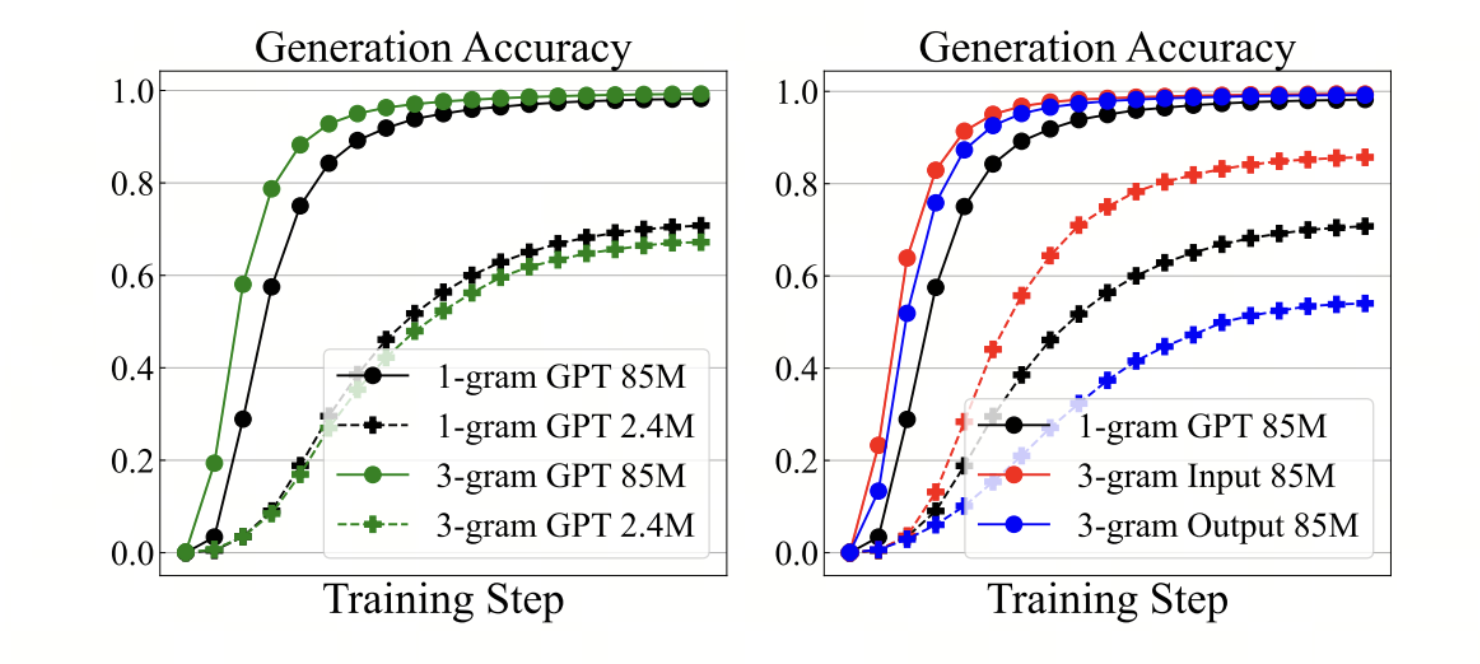
\includegraphics[width=0.9\linewidth,height=\textheight,keepaspectratio,alt={How input and output vocabulary affect models of different sizes}]{assets/over-encoding-vocabulary.png}

\end{center}

Over Encoding (OE) finds that the culprit is actually \textbf{a large
output vocabulary}.

There is an intuitive explanation. Enlarging the input vocabulary
strengthens \textbf{the mapping from context to representations}.
Enlarging the output vocabulary, however, turns prediction into a
finer-grained and more difficult classification problem. Large models
can make use of this supervision, while small models are more likely to
underfit.

From this perspective, \textbf{input vocabulary and output vocabulary
should not be tied together when scaling}.

\subsubsection{Hierarchical N-grams and Feature
Hashing}\label{hierarchical-n-grams-and-feature-hashing}

The paper keeps the original BPE token sequence unchanged. Instead of
looking up only the current token at each input position, it
\textbf{looks up both the current token and n-grams ending at that
position}.

For example, if the current token is \(c\) and the previous two tokens
are \(a,b\), it constructs:

\begin{itemize}
\tightlist
\item
  \textbf{1-gram}: \(c\);
\item
  \textbf{2-gram}: \((b,c)\);
\item
  \textbf{3-gram}: \((a,b,c)\).
\end{itemize}

\begin{NotesFormula}

Each fixed-length n-gram is first uniquely encoded as a large integer
using:

\[
f(z_1,\ldots,z_n)=\sum_{j=1}^{n}z_j V^{j-1},
\]

\end{NotesFormula}

where \(V\) is the base vocabulary size. There are theoretically \(V^n\)
combinations, so building an embedding table with \(V^n\) rows is
impractical. The authors use \textbf{feature hashing} instead: compute
\(f(\cdot)\bmod m\) and look up a table with only \(m\) rows,
\(E[f(\cdot)\bmod m]\). Different n-grams are allowed to collide in the
same row.

\begin{NotesFormula}

\textbf{Hierarchical n-grams} means using embeddings for orders
\(1+2+\cdots+n\) at the same position, rather than only a 3-gram. For
example:

\[
h_c=E_1[c]+E_2\!\left[f(b,c)\bmod m\right]
+E_3\!\left[f(a,b,c)\bmod m\right].
\]

\end{NotesFormula}

This preserves information about individual tokens, short local
combinations, and longer local combinations at the same time.

\subsubsection{Sliced Low-Dimensional
Embeddings}\label{sliced-low-dimensional-embeddings}

\begin{NotesFormula}

For each n-gram order, the authors go further than building a single
wide \(m\times d\) table. They use \textbf{sliced low-dimensional
embeddings}, splitting the same parameter budget across \(k\) narrower
tables of size \(m_i\times(d/k)\). Each lookup returns a low-dimensional
vector, which is projected back to the model dimension using
\(W_i\in\mathbb{R}^{(d/k)\times d_{\mathrm{model}}}\), and then summed:

\[
E_{\mathrm{slice}}(x)=\sum_{i=1}^{k}E_i[x\bmod m_i]W_i.
\]

\end{NotesFormula}

The key detail is that the table sizes \(m_i\) are deliberately slightly
different, such as \(m,m+2,m+4\). The same n-gram therefore receives
several different hash addresses: \(x\bmod m\), \(x\bmod(m+2),\ldots\).
Even if it collides with another n-gram in one table, it is unlikely to
collide in every table.

The result is \textbf{BPE embeddings + hierarchical n-grams ×
low-dimensional embeddings from multiple distinct hash views}, all
summed before entering an otherwise unchanged Transformer. This adds
many sparsely accessed lookup parameters with almost no additional
Transformer backbone FLOPs.

The procedure also shows that \textbf{OE's hash addresses and sparse
lookups depend only on token IDs}. They do not need to wait for
contextual hidden states, making them well suited to CPU execution or
advance computation. The Linear projections after lookup still involve
matrix operations, but even with a very large OE parameter count, each
token accesses only a few rows. Viewed this way, it is also a form of
input embedding sparsification.

\begin{Shaded}
\begin{Highlighting}[]
\NormalTok{2{-}gram (b,c)   {-}\textgreater{} hash\_i {-}\textgreater{} Emb\_i {-}\textgreater{} Linear\_i {-}\textgreater{} sum\_i {-}{-}+}
\NormalTok{3{-}gram (a,b,c) {-}\textgreater{} hash\_i {-}\textgreater{} Emb\_i {-}\textgreater{} Linear\_i {-}\textgreater{} sum\_i {-}{-}+{-}\textgreater{} SUM}
\NormalTok{1{-}gram c      {-}\textgreater{} Token Embedding {-}{-}{-}{-}{-}{-}{-}{-}{-}{-}{-}{-}{-}{-}{-}{-}{-}{-}{-}{-}{-}{-}{-}{-}+     |}
\NormalTok{                                                              v}
\NormalTok{                                                    Transformer {-}\textgreater{} LM Head}
\end{Highlighting}
\end{Shaded}

Within each n-gram branch, \(i=1,\ldots,k\) indexes the slices. Their
outputs are summed within the branch, then added to the base token
embedding.

\clearpage

\subsection{2. Per-Layer Embeddings
(PLE)}\label{per-layer-embeddings-ple}

Gemma 3n and Gemma 4 E2B / E4B all use \textbf{Per-Layer Embeddings}.

The motivation is to \textbf{reduce the backbone's burden of storing
static memories, using memory scaling in place of compute scaling},
while allowing different depths to learn different token priors.
Reducing the burden of static memory is also a motivation behind the
later Engram work.

\begin{NotesFormula}

In addition to the ordinary token embedding, each token receives an
independent low-dimensional embedding for every layer. For example:

\[
\text{token}\times\text{layer}\;\longrightarrow\;\text{256-d vector}.
\]

\end{NotesFormula}

At layer \(m\), the model retrieves the token's PLE for that layer. The
current contextual hidden state is multiplied by a gate matrix and
passed through GELU to produce a gate that selectively reads the stored
information. The result is projected back to the hidden dimension and
added to the residual stream.

This can be understood as \textbf{layer-specific token memory}. Deep
layers do not have to rely entirely on the preceding dozens of layers to
preserve the original token information. Each layer can directly access
static memory learned specifically for that depth.

This increases model capacity through a large number of sparsely
accessed embedding parameters, while adding relatively little actual
computation.

\subsection{3. Engram}\label{engram}

\subsubsection{Motivation: Conditional
Memory}\label{motivation-conditional-memory}

Engram is a rare paper that is excellent both technically and in its
writing. It builds on the design experience of OE and PLE and introduces
further innovations. Let's take a closer look.

Its motivation begins by separating model computation into two
categories:

\begin{enumerate}
\def\labelenumi{\arabic{enumi}.}
\item
  \textbf{Dynamic, compositional computation}: logical reasoning,
  mathematical derivations, code, and long-range relationships, which
  require actual computation through deep blocks.
\item
  \textbf{Static, local, repeated patterns}: names, places, fixed
  phrases, idioms, and common local combinations. These are closer to
  ``see a key, retrieve a value'' and do not require deep computation to
  obtain this kind of factual knowledge.
\end{enumerate}

\textbf{The authors have an even larger ambition: to establish a second
axis of sparsity, Conditional Memory, and a third way to scale LLM
capacity alongside dense compute and MoE experts: adding static,
sparsely accessed memory.}

\subsubsection{From N-gram Lookup to Residual
Injection}\label{from-n-gram-lookup-to-residual-injection}

\begin{center}

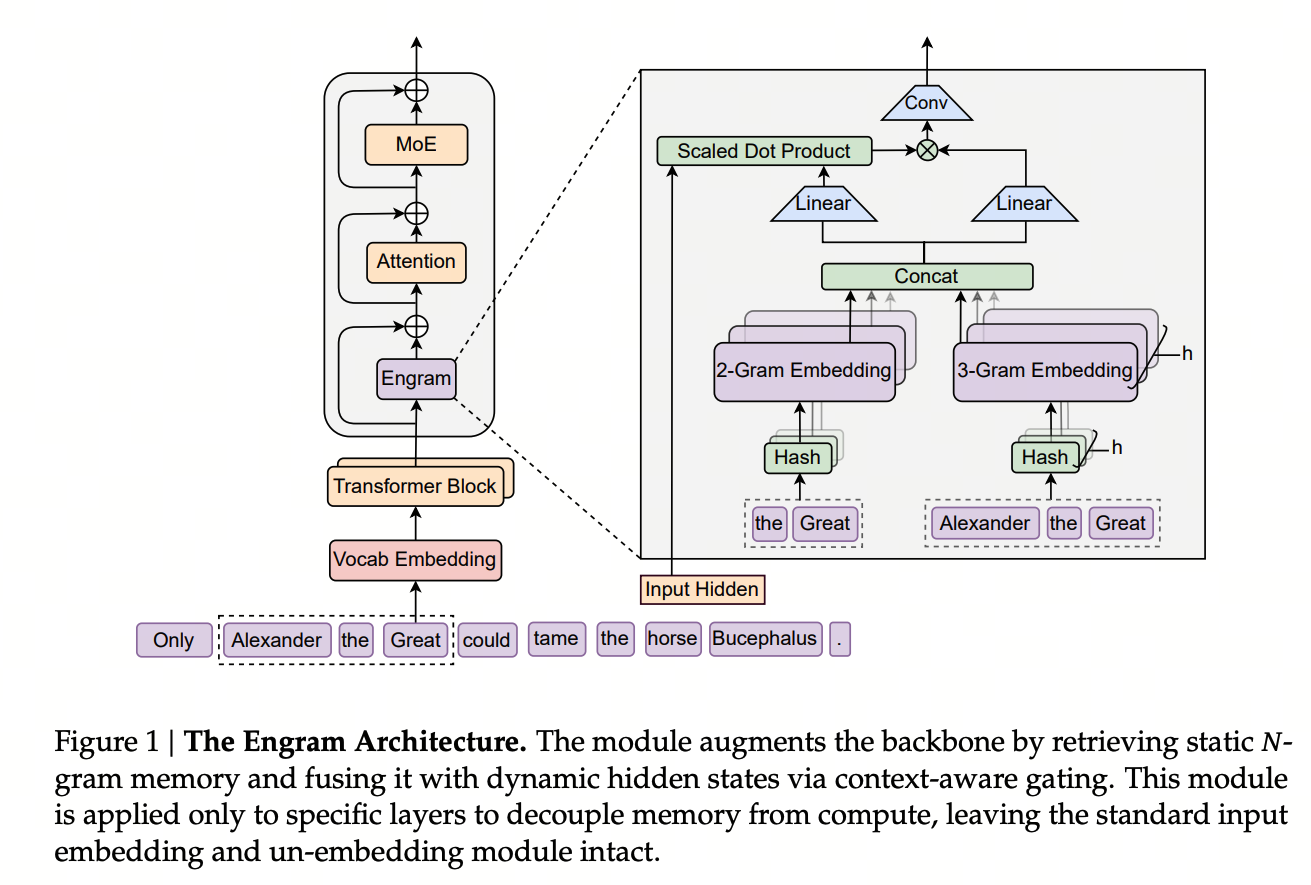
\includegraphics[width=0.9\linewidth,height=\textheight,keepaspectratio,alt={The Engram architecture and conditional memory retrieval}]{assets/engram-architecture.png}

\end{center}

Many tokens in an LLM tokenizer have \textbf{nearly equivalent textual
forms but completely different IDs}, owing to differences such as
capitalization or leading spaces. Engram first applies
\textbf{canonicalization}, mapping these variants into a more unified
representation space.

\begin{NotesFormula}

At each position, it then constructs local phrases such as 2-grams and
3-grams and uses multiple independent hash functions to retrieve entries
from very large embedding tables:

\[
e_t=\operatorname{Concat}\!\left(
\left\{E_{n,k}[\phi_{n,k}(g_{t,n})]\right\}_{n,k}
\right).
\]

\end{NotesFormula}

\begin{NotesFormula}

The retrieved memory \(e_t\) passes through a shared Value projection
\(W_V\):

\[
v_t=W_Ve_t.
\]

\end{NotesFormula}

\begin{NotesFormula}

In mHC, the residual streams within a layer share this memory and
\(W_V\), while each branch \(m\) has its own \(W_K^{(m)}\). The model
computes a \textbf{context-aware gate} from the current branch's hidden
state \(h_t^{(m)}\) and the memory key:

\[
\alpha_t^{(m)}=\sigma\!\left(
\frac{
\operatorname{RMSNorm}(h_t^{(m)})^{\top}
\operatorname{RMSNorm}(W_K^{(m)}e_t)
}{\sqrt{d}}
\right).
\]

\end{NotesFormula}

\begin{NotesFormula}

The memory actually read by that branch is then:

\[
\tilde v_t^{(m)}=\alpha_t^{(m)}v_t.
\]

\end{NotesFormula}

\begin{NotesFormula}

Finally, the paper adds a lightweight \textbf{short depthwise causal
convolution} over the gated memory sequence \(\tilde V\), with the
stated goal of expanding the local receptive field and increasing
nonlinearity:

\[
Y=\operatorname{SiLU}\!\left(
\operatorname{Conv1D}\!\left(\operatorname{RMSNorm}(\tilde V)\right)
\right)+\tilde V.
\]

\end{NotesFormula}

(I am quite skeptical about this component.)

The result \(Y\) is written back to the corresponding residual stream.
The full procedure is \textbf{canonicalization → N-gram hash lookup →
context-aware gated retrieval → local causal convolution refinement →
residual injection}.

\subsubsection{Infrastructure: Host Memory and
Prefetch}\label{infrastructure-host-memory-and-prefetch}

As with OE, hash addresses depend only on token IDs. Memory can
therefore be looked up in CPU / host DRAM in advance and transferred
asynchronously to the GPU, overlapping with earlier-layer computation.
Parameter capacity can grow substantially while the number of lookups
per token stays fixed; projections, gating, and convolution still incur
a small computational cost.

\begin{center}

\pandocbounded{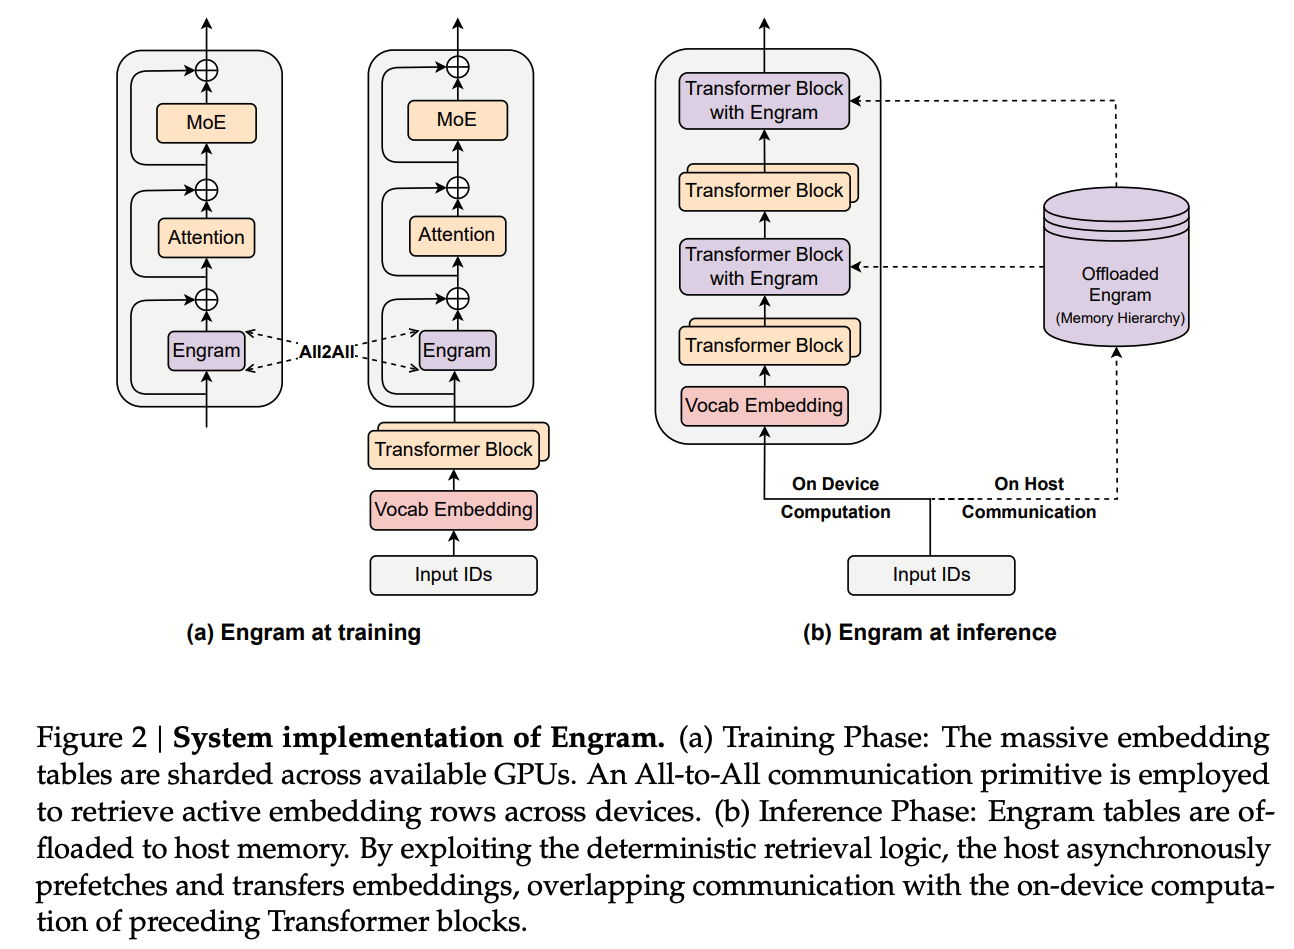
\includegraphics[keepaspectratio,alt={Engram system implementation during training and inference}]{assets/engram-system.png}}

\end{center}

\clearpage

\subsubsection{Interesting Experimental Questions and
Findings}\label{interesting-experimental-questions-and-findings}

The results speak for themselves. Let's look at some of the more
interesting experimental questions and conclusions in the paper.

\begin{enumerate}
\def\labelenumi{\arabic{enumi}.}
\item
  \textbf{How should a fixed parameter budget be split between MoE and
  Engram?}

  The experiments hold total and active parameter counts fixed, changing
  only how the sparse budget is allocated between MoE and Engram. The
  result is clearly U-shaped: pure MoE is not optimal. Allocating
  roughly \textbf{75\%-80\% to MoE and 20\%-25\% to Engram} works best.
\item
  \textbf{Can Engram scale?}

  Yes. With the backbone fixed, progressively enlarging the Engram table
  keeps reducing validation loss, with a relatively stable scaling
  trend. Even better, the memory table can become very large while each
  token still accesses a fixed number of rows, so parameter growth does
  not produce a proportional increase in FLOPs. Memory size can
  therefore become a new scaling axis independent of model computation.
\item
  \textbf{Can N-gram memory improve reasoning?}

  Yes! Engram itself is not ``doing reasoning,'' but it may spare early
  layers from reconstructing static entities and phrases, allowing
  higher-level semantic processing to begin earlier. LogitLens and CKA
  show that shallower layers in an Engram model can form representations
  resembling those of deeper baseline layers. The authors describe this
  as improved \textbf{effective depth}: more of the Transformer's actual
  depth is available for compositional reasoning, mathematics, and code.
\item
  \textbf{Can Engram improve long-context performance?}

  Yes! Ordinary Attention handles not only long-range dependencies but
  also considerable local pattern modeling. Engram assigns some local
  dependencies directly to memory lookup, leaving more Attention
  capacity for global dependencies. (Writing this reminds me once again
  of Zeyuan's Physics of Language Models.)
\item
  \textbf{Where should Engram be placed, and which components actually
  matter?}

  There is a trade-off. Too early, the hidden state lacks context and
  the gate may be inaccurate; too late, earlier-layer computation has
  already been spent. The paper finds that placing Engram at the second
  layer works best, and splitting the budget across multiple Engram
  modules at different depths can improve results further.

  In the ablations, \textbf{context-aware gating, tokenizer compression,
  and mHC branch-specific fusion} matter most. Short Causal Conv brings
  only a small improvement (so DS4.1 simply removes it).
\item
  \textbf{What does Engram actually learn?}

  Disabling Engram causes a large decline on factual knowledge tasks,
  while reading comprehension is better preserved. This suggests a
  natural division of labor: Engram focuses more on static parametric
  knowledge, such as entities, facts, and fixed phrases, while the
  Transformer backbone focuses more on contextual processing,
  composition, and reasoning.
\end{enumerate}

Of course, these conclusions come from experiments on small models. The
specific Engram configurations in released models have already evolved.

\clearpage

\subsection{4. Ablations in Qwen3.8 Flash
Next}\label{ablations-in-qwen3.8-flash-next}

Here, I will briefly discuss the ablation findings from Qwen3.8 Flash
Next.

\begin{center}

\pandocbounded{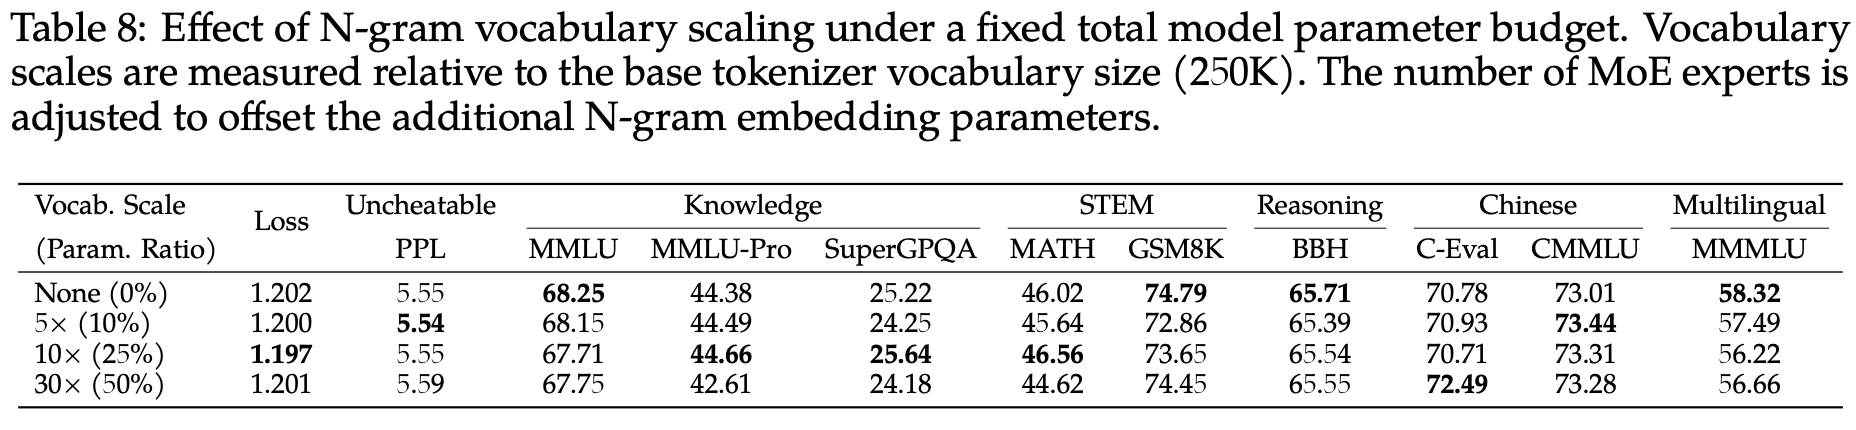
\includegraphics[keepaspectratio,alt={N-gram vocabulary scaling under a fixed total parameter budget}]{assets/qwen-fixed-budget.png}}

\end{center}

\begin{enumerate}
\def\labelenumi{\arabic{enumi}.}
\item
  \textbf{N-gram layer placement.} Shallow layers are generally
  stronger, although middle and deep layers remain competitive.
  Splitting a fixed parameter budget across two layers does not provide
  consistent gains. The final choice is therefore \textbf{Layer 2 only}.
  This allows N-gram embeddings to be prefetched from host memory while
  Layer 1 is being computed.
\item
  \textbf{Fixed total parameter budget.} Allocating about 25\% of the
  parameters to N-grams gives the best training loss, but downstream
  evaluations do not show a corresponding optimum at 25\%.
\item
  \textbf{Fixed backbone with additional N-gram parameters.} N-grams
  continue to scale in terms of loss. However, \textbf{lower loss does
  not necessarily mean better downstream performance}: reasoning
  benchmarks plateau or even decline beyond a certain memory size.
\item
  \textbf{Chinese benchmarks.} N-gram scaling is particularly consistent
  on Chinese benchmarks such as C-Eval and CMMLU.
\end{enumerate}

\begin{center}

\pandocbounded{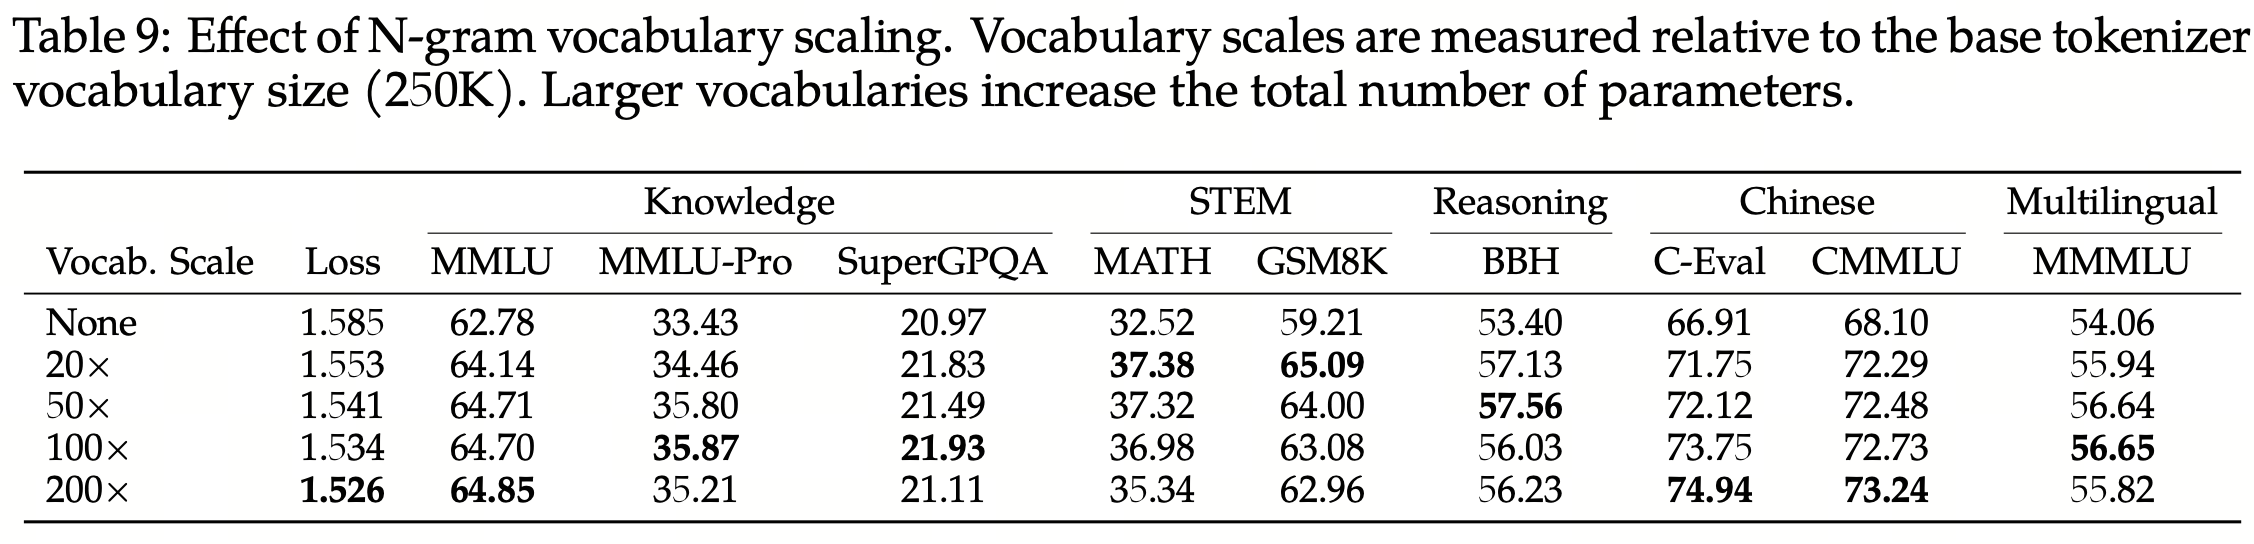
\includegraphics[keepaspectratio,alt={Scaling N-gram parameters with the backbone fixed}]{assets/qwen-memory-scaling.png}}

\end{center}

LongCat-2.0 makes somewhat different choices as well. I will not go into
them here; interested readers can consult its technical report.

\end{document}
